\begin{center}
\

\vspace{3cm}

{\fontsize{40}{0}\sffamily\bfseries Undergraduate Mathematics}

\vspace{2cm}

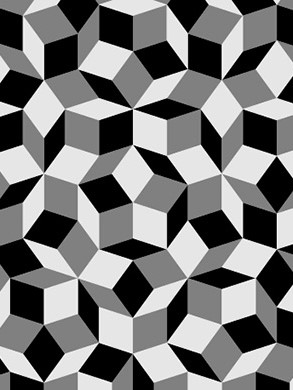
\includegraphics[width=0.6\linewidth]{images/penrose-bnw.jpg}

\vspace{2cm}

{\Huge Ryan Joo Rui An}
\nbvspace[1]
\end{center}

\thispagestyle{empty}
\pagebreak

\

\thispagestyle{empty}
\pagebreak

\begin{center}
\

\vspace{6cm}

{\huge\bfseries Undergraduate Mathematics}

\vspace{2cm}

{\huge Ryan Joo Rui An}
\end{center}
\thispagestyle{empty}
\pagebreak

\thispagestyle{empty}
\

\vfill

\begin{quote}
\textit{The mathematician does not study mathematics because it is useful; he studies it because he delights in it and he delights in it because it is beautiful.}

\begin{flushright}--- Henri Poincar\'{e} (1854--1912)\\
French mathematician and theoretical physicist\end{flushright}
\end{quote}

\vfill

Copyright \copyright \ 2024 by Ryan Joo Rui An.

This book is licensed under the terms of the Creative Commons Attribution-NonCommercial 4.0 International License (\url{https://creativecommons.org/licenses/by-nc/4.0}), which permits any noncommercial use, sharing, adaptation, distribution and reproduction in any medium or format, as long as you give appropriate credit to original author and source, provide a link to the Creative Commons license, and indicate if changes were made. The images or other third party material in this book are included in the book's Creative Commons license, unless indicated otherwise in a credit line to the material. If material is not included in the book's Creative Commons license and your intended use is not permitted by statutory regulation or exceeds the permitted use, you will need to obtain permission directly from the copyright holder.

This is (still!) an incomplete draft. Please send corrections and comments to \url{ryanjooruian18@gmail.com}, or pull-request at \url{https://github.com/Ryanjoo18/undergrad-math}.

Typeset using \LaTeX.

Last updated \today.
\pagebreak

\frontmatter
\begin{comment}
\section*{About the Author}
\textbf{Ryan Joo Rui An} is a high school student who has just completed his A-Level studies in Singapore. He has spent over 11 years honing his skills in various mathematics competitions. His journey began at an early age, where he developed a fascination with numbers while doing mental arithmetic. This early interest quickly blossomed into a deep commitment to mathematics, leading him to participate in numerous mathematics olympiads competitions.

The author's (not many) mathematics credentials include:
\begin{itemize}
\item 3 Silver awards in the \emph{Singapore Mathematics Olympiad} 2022 to 2024;
\item 6 Gold awards in the \emph{Singapore and Asian Schools Math Olympiad} 2019 to 2023, top in Singapore in 2022 and 2023, top in Malaysia in 2024;
\item Merit award in the \emph{Singapore International Mathematical and Computational Challenge} 2024;
\item 2 Prize awards, 2 High Distinction awards in the \emph{Australian Mathematics Competition} 2019 to 2023, best in school in 2023;
\item Honourable mention in the \emph{High School Mathematical Contest in Modeling} 2023;
\item 2nd place in the \emph{Hua Lo Geng Secondary School Mathematics Competition} 2019;
\item 1st place in the \emph{Chen Jingrun's Cup Secondary School Mathematics Competition} 2019.
\end{itemize}

Outside of mathematics, the author has a keen interest in playing chess and programming.

This book is a culmination of the author's years of experience, dedication, and love for mathematics while he studies mathematics at the undergraduate level.
\pagebreak
\end{comment}

\section*{Preface}
\ifabsalg
\cref{part:abstract-algebra} covers \textbf{abstract algebra}, which follows \cite{dummit-foote,artin}. \cref{chap:groups} introduces groups; \cref{chap:rings} introduces rings.
\fi

\iflinalg
\cref{part:linear-algebra} covers \textbf{linear algebra}, which follows \cite{axler}. \cref{chap:vector-spaces} introduces vector spaces, subspaces, span, linear independence, bases and dimension. \cref{chap:linear-maps} concerns linear maps and related concepts.
\fi

\ifranalysis
\cref{part:real-analysis} covers \textbf{real analysis}, which follows \cite{rudin,apostol,bartle-sherbert}. \cite{alcock} is also a good read to get some intuition into some abstract notions. \cref{chap:number-systems} introduces the real and complex number systems; \cref{chap:basic-topology} covers basic topology required for subsequent chapters; \cref{chap:num-seq-series} and \cref{chap:func-seq-series} cover numerical sequences and series, and sequences and series of functions respectively; \cref{chap:real-analysis_continuity} covers continuity of functions; \cref{chap:differentiation} and \cref{chap:rs-integration} cover differentiation and Riemann--Stieljes integration respectively; \cref{chap:special-functions} covers some special functions such as power series, exponential and logarithmic functions, trigonometric functions, fourier series and the gamma function.
\fi

\ifcanalysis
\cref{part:complex-analysis} covers \textbf{complex analysis}, which follows \cite{ahlfors,lang}.
\fi

\iftop
\cref{part:topology} covers \textbf{topology}, which follows \cite{munkres}.
\fi

\ifappend
The reader is not assumed to have any mathematical prerequisites, although some experience with proofs may be helpful. \textbf{Preliminary topics} such as logic and methods of proofs (\cref{chap:logic-proofs}), and basic set theory (\cref{chap:set-theory}) are covered in the appendix.
\fi

\subsection*{Note on Presentation}
The following are some common mathematical terms used in this book. They are neither exhaustive nor rigorous, but they should give you a good idea of what is meant when these terms are used. The following terms are \textbf{bolded} when they are used, for readability.
\begin{itemize}
\item \textbf{Definition}: a precise and unambiguous description of the meaning of a mathematical term. It characterizes the meaning of a word by giving all the properties and only those properties that must be true.
\item \textbf{Theorem}: a mathematical statement that is proved using rigorous mathematical reasoning. In a mathematical paper, the term theorem is often reserved for the most important results.
\item \textbf{Lemma}: a minor result whose sole purpose is to help in proving a theorem. It is a stepping stone on the path to proving a theorem. Very occasionally lemmas can take on a life of their own (Zorn's lemma, Urysohn's lemma, Burnside's lemma, Sperner's lemma).
\item \textbf{Corollary}: a result in which the (usually short) proof relies heavily on a given theorem (we often say that ``this is a corollary of Theorem A'').
\item \textbf{Proposition}: a proved and often interesting result, but generally less important than a theorem.
\item \textbf{Conjecture}: a statement that is unproved, but is believed to be true (Collatz conjecture, Goldbach conjecture, twin prime conjecture).
\item \textbf{Claim}: an assertion that is then proved. It is often used like an informal lemma.
\item \textbf{Axiom/Postulate}: a statement that is assumed to be true without proof. These are the basic building blocks from which all theorems are proved (Euclid's five postulates, Zermelo--Fraenkel axioms, Peano axioms).
\item \textbf{Identity}: a mathematical expression giving the equality of two (often variable) quantities (trigonometric identities, Euler's identity).
\item \textbf{Paradox}: a statement that can be shown, using a given set of axioms and definitions, to be both true and false. Paradoxes are often used to show the inconsistencies in a flawed theory (Russell's paradox). The term paradox is often used informally to describe a surprising or counterintuitive result that follows from a given set of rules (Banach--Tarski paradox, Alabama paradox, Gabriel's horn).
\end{itemize}

Important terms are \vocab{coloured} when they are first defined, and are included in the glossary at the end of the book. Less important terms are instead \emph{italicised} when they are first defined, and are not included in the glossary.

\subsection*{Note on Problem Solving}
Mathematics is about problem solving. In \cite{polya}, George P\'{o}lya outlined the following problem solving cycle.
\begin{enumerate}
\item \textbf{Understand the problem}

Ask yourself the following questions:
\begin{itemize}
\item Do you understand all the words used in stating the problem?
\item Is it possible to satisfy the condition? Is the condition sufficient to determine the unknown? Or is it insufficient? Or redundant? Or contradictory?
\item What are you asked to find or show? Can you restate the problem in your own words?
\item Draw a figure. Introduce suitable notation.
\item Is there enough information to enable you to find a solution?
\end{itemize}

\item \textbf{Devise a plan}

A partial list of heuristics -- good rules of thumb to solve problems -- is included:
\begin{multicols}{2}
\begin{itemize}
\item Guess and check
\item Look for a pattern
\item Make an orderly list
\item Draw a picture
\item Eliminate possibilities
\item Solve a simpler problem
\item Use symmetry
\item Use a model
\item Consider special cases
\item Work backwards
\item Use direct reasoning
\item Use a formula
\item Solve an equation
\item Be ingenious
\end{itemize}
\end{multicols}

\item \textbf{Execute the plan}

This step is usually easier than devising the plan. In general, all you need is care and patience, given that you have the necessary skills. Persist with the plan that you have chosen. If it continues not to work discard it and choose another. Don't be misled, this is how mathematics is done, even by professionals.

\begin{itemize}
\item Carrying out your plan of the solution, check each step. Can you see clearly that the step is correct? Can you prove that it is correct?
\end{itemize}

\item \textbf{Check and expand}

P\'{o}lya mentions that much can be gained by taking the time to reflect and look back at what you have done, what worked, and what didn't. Doing this will enable you to predict what strategy to use to solve future problems.

Look back reviewing and checking your results. Ask yourself the following questions:
\begin{itemize}
\item Can you check the result? Can you check the argument?
\item Can you derive the solution differently? Can you see it at a glance?
\item Can you use the result, or the method, for some other problem?
\end{itemize}
\end{enumerate}

Building on P\'{o}lya's problem solving strategy, Schoenfeld \cite{schoenfeld} came up with the following framework for problem solving, consisting of four components:
\begin{enumerate}
\item \textbf{Cognitive resources}: the body of facts and procedures at one's disposal.
\item \textbf{Heuristics}: `rules of thumb' for making progress in difficult situations.
\item \textbf{Control}: having to do with the efficiency with which individuals utilise the knowledge at their disposal. Sometimes, this is referred to as metacognition, which can be roughly translated as `thinking about one's own thinking'.
\begin{enumerate}
\item These are questions to ask oneself to monitor one's thinking.
\begin{itemize}
    \item What (exactly) am I doing? [Describe it precisely.] Be clear what I am doing NOW. Why am I doing it? [Tell how it fits into the solution.]
    \item Be clear what I am doing in the context of the BIG picture -- the solution. Be clear what I am going to do NEXT.
\end{itemize}

\item Stop and reassess your options when you
\begin{itemize}
    \item cannot answer the questions satisfactorily [probably you are on the wrong track]; OR
    \item are stuck in what you are doing [the track may not be right or it is right but it is at that moment too difficult for you].
\end{itemize}

\item Decide if you want to
\begin{itemize}
    \item carry on with the plan,
    \item abandon the plan, OR
    \item put on hold and try another plan.
\end{itemize}
\end{enumerate}

\item \textbf{Belief system}: one's perspectives regarding the nature of a discipline and how one goes about working on it.
\end{enumerate}
\pagebreak

\tableofcontents
\pagebreak
%\printglossary[type=\acronymtype]